\begin{frame}{Hiérarchie mémoire}
	\begin{columns}[c]
		\begin{column}{.5\textwidth}
			\begin{figure}[h!]
				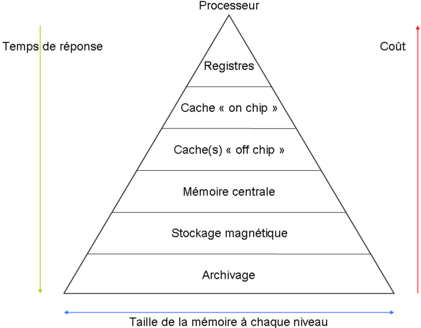
\includegraphics[scale=.35]{images/hierarchy.png}
			\end{figure}
		\end{column}
		\begin{column}{.5\textwidth}
			\begin{block}{Objectif}
				\begin{itemize}
					\item{Trouver un bon compromis entre vitesse et coût}
				\end{itemize}
			\end{block}
		\end{column}
	\end{columns}
	\begin{columns}[c]
		\begin{column}{.6\textwidth}
			\begin{block}{Hiérarchie de caches}
				\begin{itemize}
					\item{Plusieurs niveaux de cache}
					\item{Caches inclusifs/exclusifs}
				\end{itemize}
			\end{block}
		\end{column}
		\begin{column}{.4\textwidth}
			\begin{figure}[h!]
				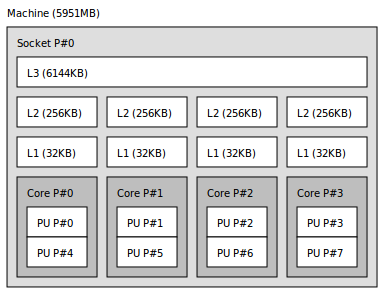
\includegraphics[scale=.3]{images/lstopo.png}
			\end{figure}
		\end{column}
	\end{columns}
\end{frame}


\begin{frame}{Recherche d'une donnée dans le cache}
	Caches organisés par ligne. 1 ligne <=> 1 étiquette = 1 adresse mémoire
	\begin{figure}[h!]
		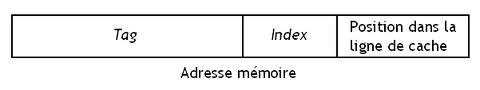
\includegraphics[scale=.3]{images/etiquette.jpeg}
	\end{figure}
	
	\begin{block}{\emph{Cache hit} et \emph{cache miss}}
		\begin{itemize}
			\item{Si le processeur trouve la donnée recherchée dans le cache : il fait un \emph{hit}}
			\item{Sinon, la donnée est rapatriée à partir de la mémoire de niveau supérieur : c'est un \emph{miss}}			
			\end{itemize}
	\end{block}
\end{frame}	

\begin{frame}{Associativité}
	\begin{block}{Fonction de correspondance adresse mémoire / cache}
		\begin{itemize}
			\item{Direct associative}
			\item{Fully associative}
			\item{k-ways associative}
		\end{itemize}
	\end{block}
	\begin{figure}[h!]
		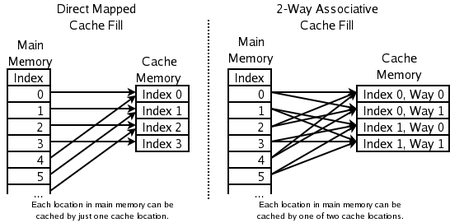
\includegraphics[scale=.33]{images/associative.png}
	\end{figure}
\end{frame}

\begin{frame}{Remplacement}
	\begin{block}{Comment ajouter une donnée dans set plein ?}
		Il existe différentes politiques de remplacement
		\begin{itemize}
			\item{FIFO (Supprimer la plus ancienne)}
			\item{LFU (Supprimer la moins utilisée)}
			\item{LRU (Supprimer la plus anciennement utilisée)}
		\end{itemize}
		En général, les données évincées sont déplacées vers la mémoire de niveau supérieur
	\end{block}
\end{frame}

\begin{frame}{Hiérarchie de caches et problèmes de cohérence}
	\begin{block}{Gestion des données entre différents niveaux}
		\begin{itemize}
			\item{\emph{Write-through} : Une donnée modifiée est tout de suite reportée aux niveaux supérieurs}
			\item{\emph{Write-back} : Le report est fait à l'éviction du cache}
		\end{itemize}
	\end{block}
	\begin{block}{Gestion des données entre caches de même niveau}
		Nécéssité d'un protocole de cohérence
	\end{block}
\end{frame}
